\documentclass{report}
\usepackage{listings}
\usepackage{graphicx}
\usepackage{hyperref}
\graphicspath{{./images}}
\def\weight{0.7}

\title{Report on CNN/Scattering classification comparison}
\author{Alberto Carli \and Gabriele Roncolato \and Leonardo Zecchin }
\date{}

\begin{document}
\maketitle
\tableofcontents
\pagebreak

\chapter{Introduction}
This document illustrates the project valid for the Visual Intelligence class of the academic year 2022/2023. \\
The assignment tests the knowledge gained in class by applying signal analysis methods, in particular we classified signals by using \textbf{Convolutional Neural Networks} and wavelet theory, specifically  \textbf{Wavelet Scattering}. \\
In this project we implemented the code necessary to classify a given dataset first by training and testing a CNN, then by applying the Wavelet Scattering Transform and training a NN with the extracted features.
Finally we compared the results obtained with these two methods in terms of accuracy against how many epochs were used to train the classifiers. \\
For the entire project, we followed the guidelines given during the laboratory lectures.


\chapter{Objectives}
The goal of this project is to explore the use of scattering transforms to improve the performance of neural networks on a given dataset.\\
Specifically, we aimed to compare the performance of a CNN trained on the original dataset to a NN trained on the scattering decomposition of the data.\\

We then visualized the filters learned by the CNN and compared them to the ones applied by the scattering transform to gain insight into the types of features that were extracted.
By accomplishing these objectives we hoped to gain a better understanding of how the CNN learns which features to extract.

\chapter{Dataset}
We used a dataset consisting of 128x128 RGB images divided into two categories: dogs and flowers. There are 1600 pictures of dogs and 1387 pictures of flowers.
We converted everything to grayscale with each class n its specific folder and every file numbered.

\chapter{Framework}
\section{Convolutional Neural Network}
\subsection{What is a CNN}
A Convolutional Neural Network (\textbf{CNN}) is a type of deep learning algorithm commonly used for image recognition and computer vision tasks. It is designed to automatically learn and extract relevant features from input images through convolutional and pooling layers, followed by fully connected layers that produce output predictions. \\
The \texttt{CNN\_128x128} architecture consists of four \textbf{convolutional} layers and three fully connected layers. The first layer takes an input image with \texttt{input\_channel} number of channels, and the output of the last layer is a vector with \texttt{num\_classes} elements representing the probability of each class.

\subsection{Architecture}
\begin{lstlisting}[language=bash]
CNN_128x128(
    (conv1): Conv2d(1, 16, kernel_size=(7, 7), stride=(2, 2), padding=(1, 1))
    (conv2): Conv2d(16, 32, kernel_size=(5, 5), stride=(2, 2), padding=(1, 1))
    (conv3): Conv2d(32, 64, kernel_size=(3, 3), stride=(2, 2), padding=(1, 1))
    (batchnorm1): BatchNorm2d(16, eps=1e-05, momentum=0.1, affine=True, track_running_stats=True)
    (batchnorm2): BatchNorm2d(32, eps=1e-05, momentum=0.1, affine=True, track_running_stats=True)
    (batchnorm3): BatchNorm2d(64, eps=1e-05, momentum=0.1, affine=True, track_running_stats=True)
    (drop1): Dropout(p=0.2, inplace=False)
    (flat): Flatten(start_dim=1, end_dim=-1)
    (fc1): Linear(in_features=256, out_features=64, bias=True)
    (drop2): Dropout(p=0.5, inplace=False)
    (fc2): Linear(in_features=64, out_features=2, bias=True)
    )
\end{lstlisting}
The model is named \texttt{CNN\_128x128} and takes as input an image with a width and height of 128 pixels and a number of channels specified by the \texttt{input\_channel} parameter
(typically 3 for RGB images or 1 for grayscale images). The number of output classes is specified by the \texttt{num\_classes} parameter.\\
The CNN consists of three \textbf{convolutional layers} with increasing numbers of output channels (16, 32, and 64, respectively). Each convolutional layer is followed by a \textbf{batch normalization layer},
a \textbf{ReLU} activation function, and a \textbf{max pooling layer} with a kernel size of 2 and a stride of 2. \\
The output of the final convolutional layer is flattened into a vector and passed through two \textbf{fully connected} (FC) layers with 64 and \texttt{num\_classes} output units, respectively.
The FC layers are followed by dropout layers to prevent overfitting.\\

During the forward pass, input images are passed through the convolutional layers, normalized and pooled before being flattened and passed through the FC layers.
The output of the last FC layer is a probability distribution over the \texttt{num\_classes} output classes, which can be used to make predictions about the input image's class.


\section{Neural Network}
\subsection{Wavelet scattering}
\subsubsection{What is a wavelet scattering}
Wavelet scattering is a mathematical technique for analyzing signals, such as sound or images, by decomposing them into different frequency bands and time scales. It works by applying a series of wavelet transforms to the signal, which effectively "filters" the signal into its constituent frequency components.\\
The key idea behind wavelet scattering is to create a representation of the signal that is invariant to translations and rotations. This allows us to extract features from the signal that are robust to changes in scale and position.
\subsubsection{How we do it}
Initially, we tried to use the Python library \textbf{Kymatio} to implement \textbf{2D wavelet scattering}, but then we decided to implement 
it through \textbf{MATLAB} because it allows us to specify scattering \textbf{parameters} better. We connected MATLAB to \textbf{Python} using 
the \textbf{matlab.engine} library. This is implemented in the \texttt{scatter\_helper.py} file.\\

The purpose of the \texttt{get\_scatterNet.m} file is to create a \textbf{scattering network} MATLAB object for input images using 
 \textbf{Wavelet Scattering transform}.\\
The function calls the \texttt{waveletScattering2} MATLAB function, which is part of the Deep Learning Toolbox. WaveletScattering2 computes the scattering coefficients for a given image using a wavelet transform, which is then used to construct the scattering network. \\
The input arguments of the \texttt{get\_scatterNet} function are used to configure the waveletScattering2 function. Specifically, \texttt{invariance\_scale} specifies the scale of invariance of the scattering coefficients, \texttt{quality\_factors} specifies the quality factors for the wavelet transform, \texttt{num\_rotations} specifies the number of rotations used in the wavelet transform, and \texttt{images\_size} specifies the size of the input image.\\
Finally, the function returns the computed scattering network as \textbf{sn}.\\

Moreover, we have incorporated the \texttt{scattering.m} file that calculates the \texttt{scatter} function. This function applies the 
\textbf{Scatter Transform} to all images passed as an input argument \texttt{images}, using the Matlab method \texttt{scatteringTransform}. \\
The \texttt{scatteringTransform} function computes the scattering transform for the input data, utilizing the provided scattering network 
(\texttt{sn}).\\

Finally, we reshaped the extracted features to keep only the highest-order scattering coefficients, after finding that our initial attempt 
to take the mean of the scattering coefficients over the spatial dimensions did not yield interesting results. We also found that keeping 
all the coefficients gave even worse results.


\subsection{Architecture}
\begin{lstlisting}[language=bash]
    NN_128x128(
      (flat): Flatten(start_dim=1, end_dim=-1)
      (fc1): Linear(in_features=40960, out_features=64, bias=True)
      (drop2): Dropout(p=0.5, inplace=False)
      (fc2): Linear(in_features=64, out_features=2, bias=True)
    )
    \end{lstlisting}
This is a neural network with \textbf{fully-connected layers} designed for image classification tasks. Unlike Convolutional Neural Networks (CNNs), 
which are commonly used for image classification, this network does not have any convolutional layers. \\
The input to the network is an image with \texttt{input\_channel} number of channels and size 128x128 pixels. The image is flattened into a vector 
using the\texttt{nn.Flatten()} layer, and then passed through two \textbf{fully-connected layers}. The first fully-connected layer has 64 nodes, 
and the second (output) layer has \texttt{num\_classes} units, which correspond to the number of classes in the classification task.\\

The \textbf{forward method} defines the forward pass of the network, which simply applies the two fully-connected layers to the input vector, with ReLU activation applied to the output of the first layer and a dropout layer applied after the ReLU activation.

\section{Pipeline}
Which model to run can be specified when calling \texttt{configurable\_classification.classify()} and passing \texttt{True} to
the parameters \textit{cnn} and \textit{nn} respectively.\\

Each model is handled separately, each execution with its own quirks, as specified in the architecture section.
Generally the pipeline involves:
\begin{enumerate}
  \item dataset preparation
  \item train-test splitting
  \item eventual augmentation
  \item train-validation splitting (eventually through k-fold)
  \item training
  \item validation
  \item testing
\end{enumerate}

In many points of the pipeline, behavior is controlled through parameters, which are written in the file \textit{parameters.yaml}.\\
These parameters are overwritten at every execution by running the script \textit{lib/scripts/make\_settings.py}.\\
Scatter-specific parameters are too, written by the same script, but to another file named \textit{scatter\_parameters.yaml}.\\

Execution results are produced as graphs of training and testing and saved in the folder \textit{results} folder, each execution in its specific folder, numbered incrementally
with the runs. The dump of the whole parameters file is saved as well.\\
The output is a figure with the training and validation loss and accuracy, for every fold,
a figure with the confusion matrices, side by side and a figure with the filters developed by the CNN, if present.
If the parameter \textit{display} is set to \texttt{True}, then graphs are displayed after execution too.\\

\subsection{Dataset preparation}
We created a class that handles the dataset \texttt{data\_handler.py}. This class provides functionality to load the dataset from the disk, subsample it, and split it
into training, validation, and test sets, wrap it into a batcher class from pytorch, transfer it to the GPU, and perform data augmentation. \\
Every random operation is seeded with 42 to ensure reproducibility.\\

When the data is loaded from disk, every class folder is read with the \texttt{cv2.imread()} function and a list of labels is generated assigning a number to the class, incrementally. \\
Then if the parameter \texttt{samples} is set (e.g. not None), the dataset is subsampled by randomly selecting an equal amount of images from each class up to the \texttt{samples} value specified. \\
The dataset and labels are saved as class attributes and returned as \texttt{pytorch.Tensor()}.\\

The dataset is then split into training, validation, and test sets using the \texttt{get\_data\_split()} function, which is just a wrapper for the \texttt{train\_test\_split()} function from \texttt{sklearn.model\_selection} to 
better handle the data and seed it with a constant seed (42). \\
The \texttt{test\_perc} parameter controls the percentage of split between train and test sets by specifying how much. \\

Then, if the folds parameter is set to more than 1, the training set is split and iterated through \texttt{folds} folds using the \texttt{sklearn.model\_selection.KFold()}. \\
Otherwise, the training set is split into training and validation sets using the \texttt{train\_test\_split()} function from \texttt{sklearn.model\_selection} with 0.2 of the dataset going to validation. \\
The validation set is used to monitor the training process and to detect overfitting. \\

\subsection{Augmentation}
The \texttt{data\_handler} class provides a method to perform data augmentation on the dataset. Again, this is just a wrapper function for some \texttt{torchvision.transforms} 
all linked to a policy selected in the code. Aternative (or custom) policies can be found in the file \texttt{lib/scripts/custom\_augment.py}. \\

The augmentation is performed by randomly applying a series of transformations to the images in the dataset. Our policy consists in random rotation of angles between 0 and 90 degrees.\\

In our pipeline, the transformations are applied to the training set only, before being split into training and validation sets, while the testing set is not augmented. \\
The original image is kept and then a number of new augmented images is generated as specified in the parameter \texttt{augmentations}.\\

\subsection{Training}
The training procedure is shared between the two models. \\
The training is performed by the \texttt{train()} function in the \texttt{lib/train\_test.py} file. \\

Two optimizers can be selected with the \texttt{optimizer} parameter: \texttt{0} = \texttt{SGD} or \texttt{1} = \texttt{Adam} to which are given parameters
as required. SGD uses \textit{learning\_rate} and \textit{momentum}, while Adam uses only \textit{learning\_rate}. \\
\textit{Cross Entropy} is used as loss function. \\

The training is performed by iterating through the training set \texttt{epochs} times. \\
The function expects the dataset as a \texttt{torch.utils.data.DataLoader} and iterates by batch alternating classification, loss calculation and backpropagation.\\

If a GPU is available (and detected by pytorch), each batch will be loaded onto GPU and training will happen there. \\
The training is monitored by printing the loss and accuracy on the training set every epoch. \\
Training accuracy and loss are stored into lists and then returned after the training is done, to be used for plotting. \\

\subsection{Validation}
Validation can be enabled by setting the \texttt{epoch\_val} parameter to a positive number, or disabled entirely by giving it value \texttt{None}.
If enabled, the validation is performed every \texttt{epoch\_val} epochs. \\

The validation is performed by setting the model to evaluation mode and running the model while iterating through the validation set. \\
A loss is calculated, but no backpropagation is performed.\\
If a GPU is available (and detected by pytorch), each batch will be loaded onto GPU and training will happen there. \\

The validation is monitored by printing the loss and accuracy on the validation set every time it is run. \\
Validation accuracy and loss are stored into lists and then returned after the training is done, to be used for plotting. \\
\subsection{Testing}
Testing is performed by the \texttt{test()} function in the \texttt{lib/train\_test.py} file. \\
The function expects the dataset as a \texttt{torch.utils.data.DataLoader} and iterates by batch, classifying each image and storing the results. \\
Basically like validation, but with testing data. In case of data augmentation, testing data is NOT augmented.\\

If a GPU is available (and detected by pytorch), each batch will be loaded onto GPU and testing will happen there. \\

Testing predictions and real results are stored and returned after testing is done, to enable more flexible analysis and metrics calculation.\\
In our case, the \texttt{metrics} class handles calculation of statistics and plotting of useful graphs.\\

\chapter{Results}
The project started from the RGB dataset images and with the models as seen during laboratory lectures.\\
We started by using the Convolutional Neural Network (CNN) model provided during laboratory lectures from which we extracted the fully connected
section and thus defined the \textbf{NN\_128x128} model.\\
These models were using RGB images, but after a short while we converted everything to grayscale images.\\

We started working with the parameters as given in the laboratory lectures, together with the models.

\section{COSA INSERIRE (Da togliere)}
\begin{itemize}
  \item trovati parametri ottimali per la scatter
  \item ma la cnn non partiva: i dati erano pochi
  \item provato a modificare la struttura della cnn (overfitting)(batchnorm, dropout, ecc)
  \item alla fine siamo riusciti ad avere buoni risultati con l'Augmentation
  \item provato autoaugment, solo traslazioni e solo rotazioni
\end{itemize}

\section{Tuning scatter}
In this first part of the study, we focused on the NN model with wavelet scattering. \\
We started by tuning the parameters of the scattering transform, which are the invariance scale $J$, the order of scattering $Q$, the number of rotations $R$, and the quality factors $Q$. \\

But using kymatio, we found that the library does not support the quality factors, so, after a bit of fruitless parameter tuning, 
we opted to use the \texttt{scattering2d} function from \texttt{kymatio.scattering2d} instead, for better control. \\

\section{Models tuning}
Then we tried to tune the parameters of the optimizer of the models.\\
We tried different learning rates and momentum values for the SGD optimizer, and finally found a combination that led to the networks actually learning.
\begin{itemize}
  \item \textbf{Learning rate}: $0.01$ 
  \item \textbf{Momentum}: $0.5$
\end{itemize}

So, in this situation we could actually try and find some good values for the MATLAB scatter transform:
\begin{itemize}
  \item \textbf{Invariance scale}: $J=6$
  \item \textbf{Order of scattering}: $2$
  \item \textbf{Number of rotations}: $[8, 8]$
\end{itemize}
We found that with these values, the neural network performed well with TODO accuracy.\\

\section{CNN}
With the scatter sorted, we now focused on the CNN model, ready to find new, different, parameters that would better suit the different model.\\
We found out that the CNN model was not learning at all, so we tried to change the structure of the model, adding Batch Normalization and Dropout layers,
as well as adding/reducing layers size and number.\\
In the meantime, through testing, we figured that the best parameters for the SGD optimizer were the following:
\begin{itemize}
  \item \textbf{Learning rate}: $0.005$ 
  \item \textbf{Momentum}: $0.9$
\end{itemize}
We also tried to use the Adam optimizer, but the results were not as good as with SGD.\\

Even though the accuracy was good, the filters were not quite what we expected (something like edge detection), so we tried to change parameters
of the model, but we observed some sort of tradeoff between the training curves (loss and accuracy) and the quality of the filters.\\
TODO sicuro dell'ordine delle cose?

\section{Augmentation}
We managed to get both reasonable training curves and good filters by using data augmentation.\\
We tried to use the \texttt{autoaugment} function from \texttt{torchvision.transforms}, and it gave very nice results.\\

But we didn't yet understand why, so we tried to use only a single type of transformation at a time and try to understand what was happening.\\
Notably, when augmentation involved only translations, the filters presented some sort of weird black edge around, so we figured they didn't help much.\\

Finally, we tried to use only rotations, and the results were very good: we could see both good edge filters and decent training curves.\\
Moreover, model's accuracy was very good, with TODO accuracy.\\
We also noticed some sort of positive correlation between the number of augmented (rotated) images and the accuracy of the model.\\



\section{Summary}
We start using the RGB images but we switch to grayscale images because the results are better. (BOH)\\
In this study, we initially used the Convolutional Neural Network (CNN) model provided during laboratory
lectures as a baseline and compared its performance to that of the Neural Network (NN) model with wavelet scattering.
We then sought to improve the results of both models by experimenting with different sets of parameters, with a particular
focus on the NN and wavelet scattering parameters. \\
These are the best parameters we found for the NN models:
\begin{itemize}
  \item \textbf{Invariance scale}: $J=6$
  \item \textbf{Order of scattering}: $2$
  \item \textbf{Number of rotations}: $[8, 8]$
  \item \textbf{Quality factors}: $[2, 1]$
  \item \textbf{Learning rate}: $0.005$ 
  \item \textbf{Momentum}: $0.9$
\end{itemize}
After identifying the best parameters, we directed our attention to the CNN model.
Our findings revealed that the dataset was relatively small, and the loss and validation
graphs suggested that the model was overfitting. To address this issue, we restructured the
CNN model by introducing BatchNorm and Dropout layers, although
the results were unsatisfactory, suggesting that these changes alone were insufficient.
o address the overfitting issue, we incorporated data augmentation into the training set,
which significantly improved the results. \\
Our attempts to augment the dataset using translations and rotations were initially promising,
but we found that the CNN filters were learning the black band generated by the transformations.
To avoid this, we opted to limit rotations to between -45 and 45 degrees.\\
\begin{itemize}
  \item \textbf{batch\_size}: 64
  \item \textbf{test\_perc}: 0.2
  \item \textbf{num\_samples}: 500
  \item \textbf{epoch\_val}: 1
  \item \textbf{num\_k\_folds}: 3
  \item \textbf{augmentations}: 16 (number of augmented images per original image)
  \item \textbf{weight\_decay}: 0.01
  \item \textbf{optimizer}: 0 (0- SGD, 1- Adam)
  \item \textbf{learning\_rate}: 0.005 (scale for how much new weights are evaluated)
  \item \textbf{momentum}: 0.9 (scale for past experience to not be perturbed by new ones)
  \item \textbf{num\_epochs}: 200
\end{itemize}
\pagebreak
\chapter{Conclusions}

Our study has revealed several key findings regarding the impact of parameter selection and data augmentation 
techniques on the performance of Convolutional Neural Networks (CNNs) and Neural Networks (NNs). The optimal 
parameters varied between the two models, but our results suggest that rotations were the most effective 
parameter for improving performance. However, the reasons for this improvement are not entirely clear, as it is 
uncertain whether it is due to the rotations themselves or the increase in the number of training examples. 
While using more samples can lead to a training process that is noisier and with "faded" filters, it can also 
result in better generalization. Indeed, data augmentation techniques such as rotations can produce filters that 
are more generalizable to unseen data, as the model learns to identify more robust features that are less 
dependent on specific input configurations. Nonetheless, it is crucial to find the right balance between the 
number and type of augmented samples and the complexity of the model to avoid overfitting. Overall, our findings 
highlight the importance of careful parameter selection and the potential benefits of using rotation as a data 
augmentation technique for improving the performance and generalization of CNNs and NNs.

\pagebreak

\part{Appendix}
\appendix

\section{Executions}
AGGIUNGERE LE VARIE ESECUZIONI CON IMMAGINI\\

These are the results obtained with the best parameters found for the CNN model:
\begin{figure}[ht!]
  \centering
  \begin{minipage}[b]{0.7\linewidth}
    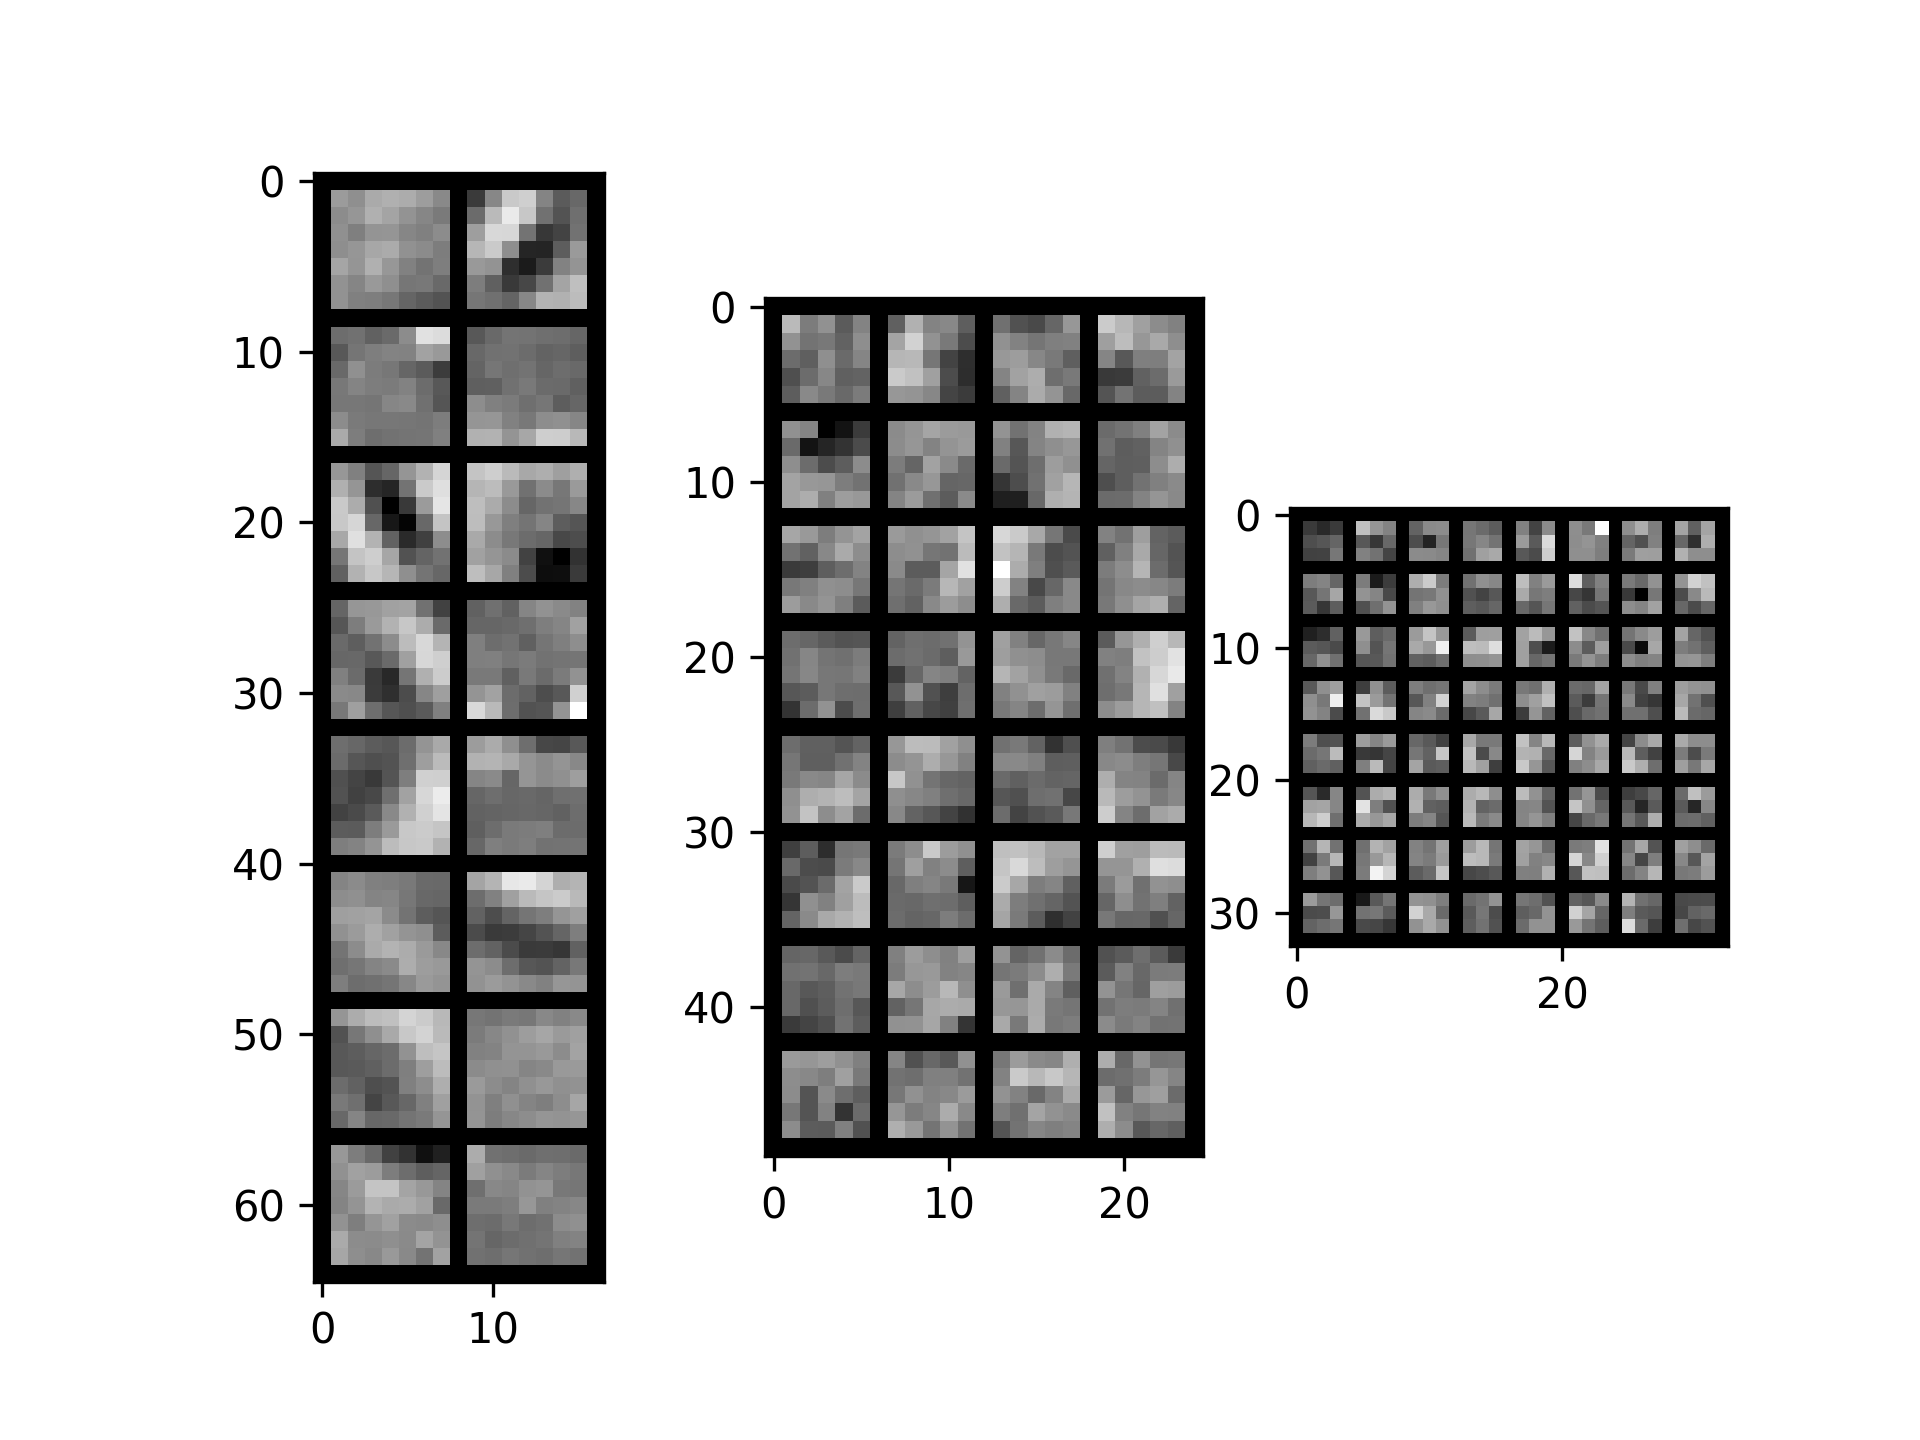
\includegraphics[width=\linewidth]{3.CNN_500_sample/CNN_filters.png}
    \caption{CNN filters.}
    \label{fig:image1}
  \end{minipage}
  \hspace{0.5cm}
  \begin{minipage}[b]{0.7\linewidth}
    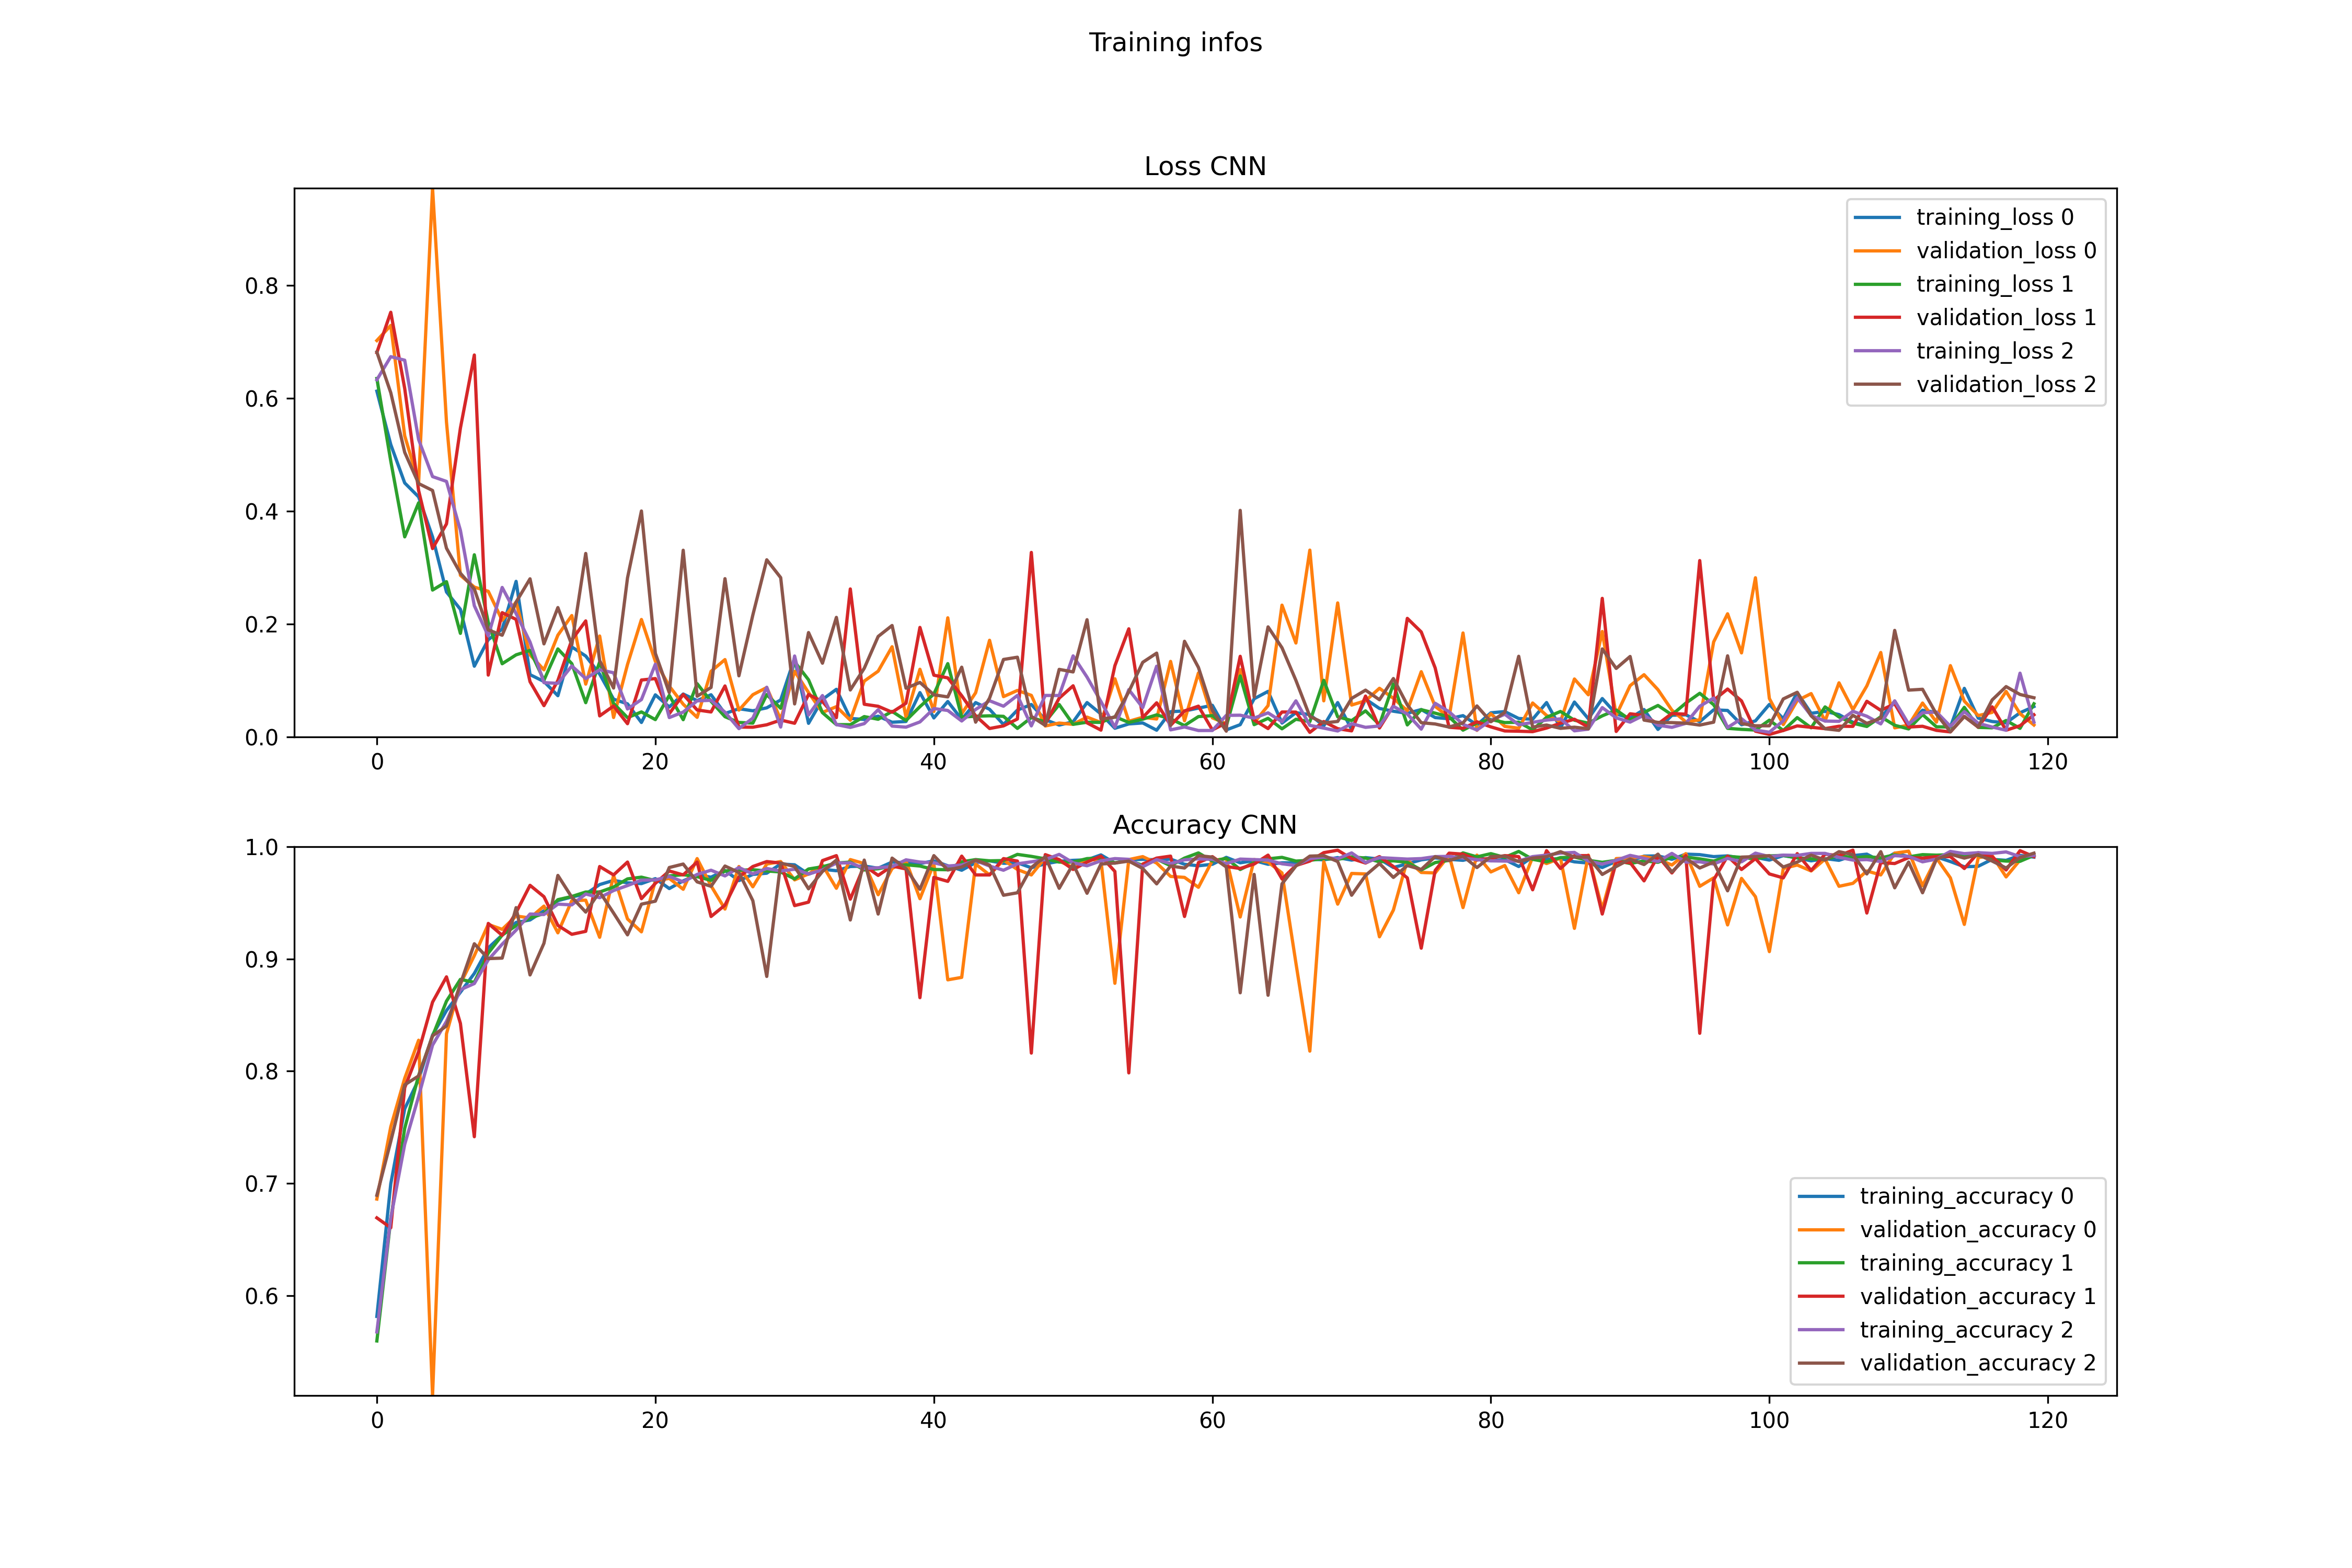
\includegraphics[width=\linewidth]{3.CNN_500_sample/training_infos.png}
    \caption{Loss and Validation graphs.}
    \label{fig:image2}
  \end{minipage}
\end{figure}\\
The \textbf{accuracy} reached in test is $0.82$.\\
\pagebreak

The we tried with more samples ($2500$) and these are the results:\\
\begin{figure}[ht!]
  \centering
  \begin{minipage}[b]{\weight\linewidth}
    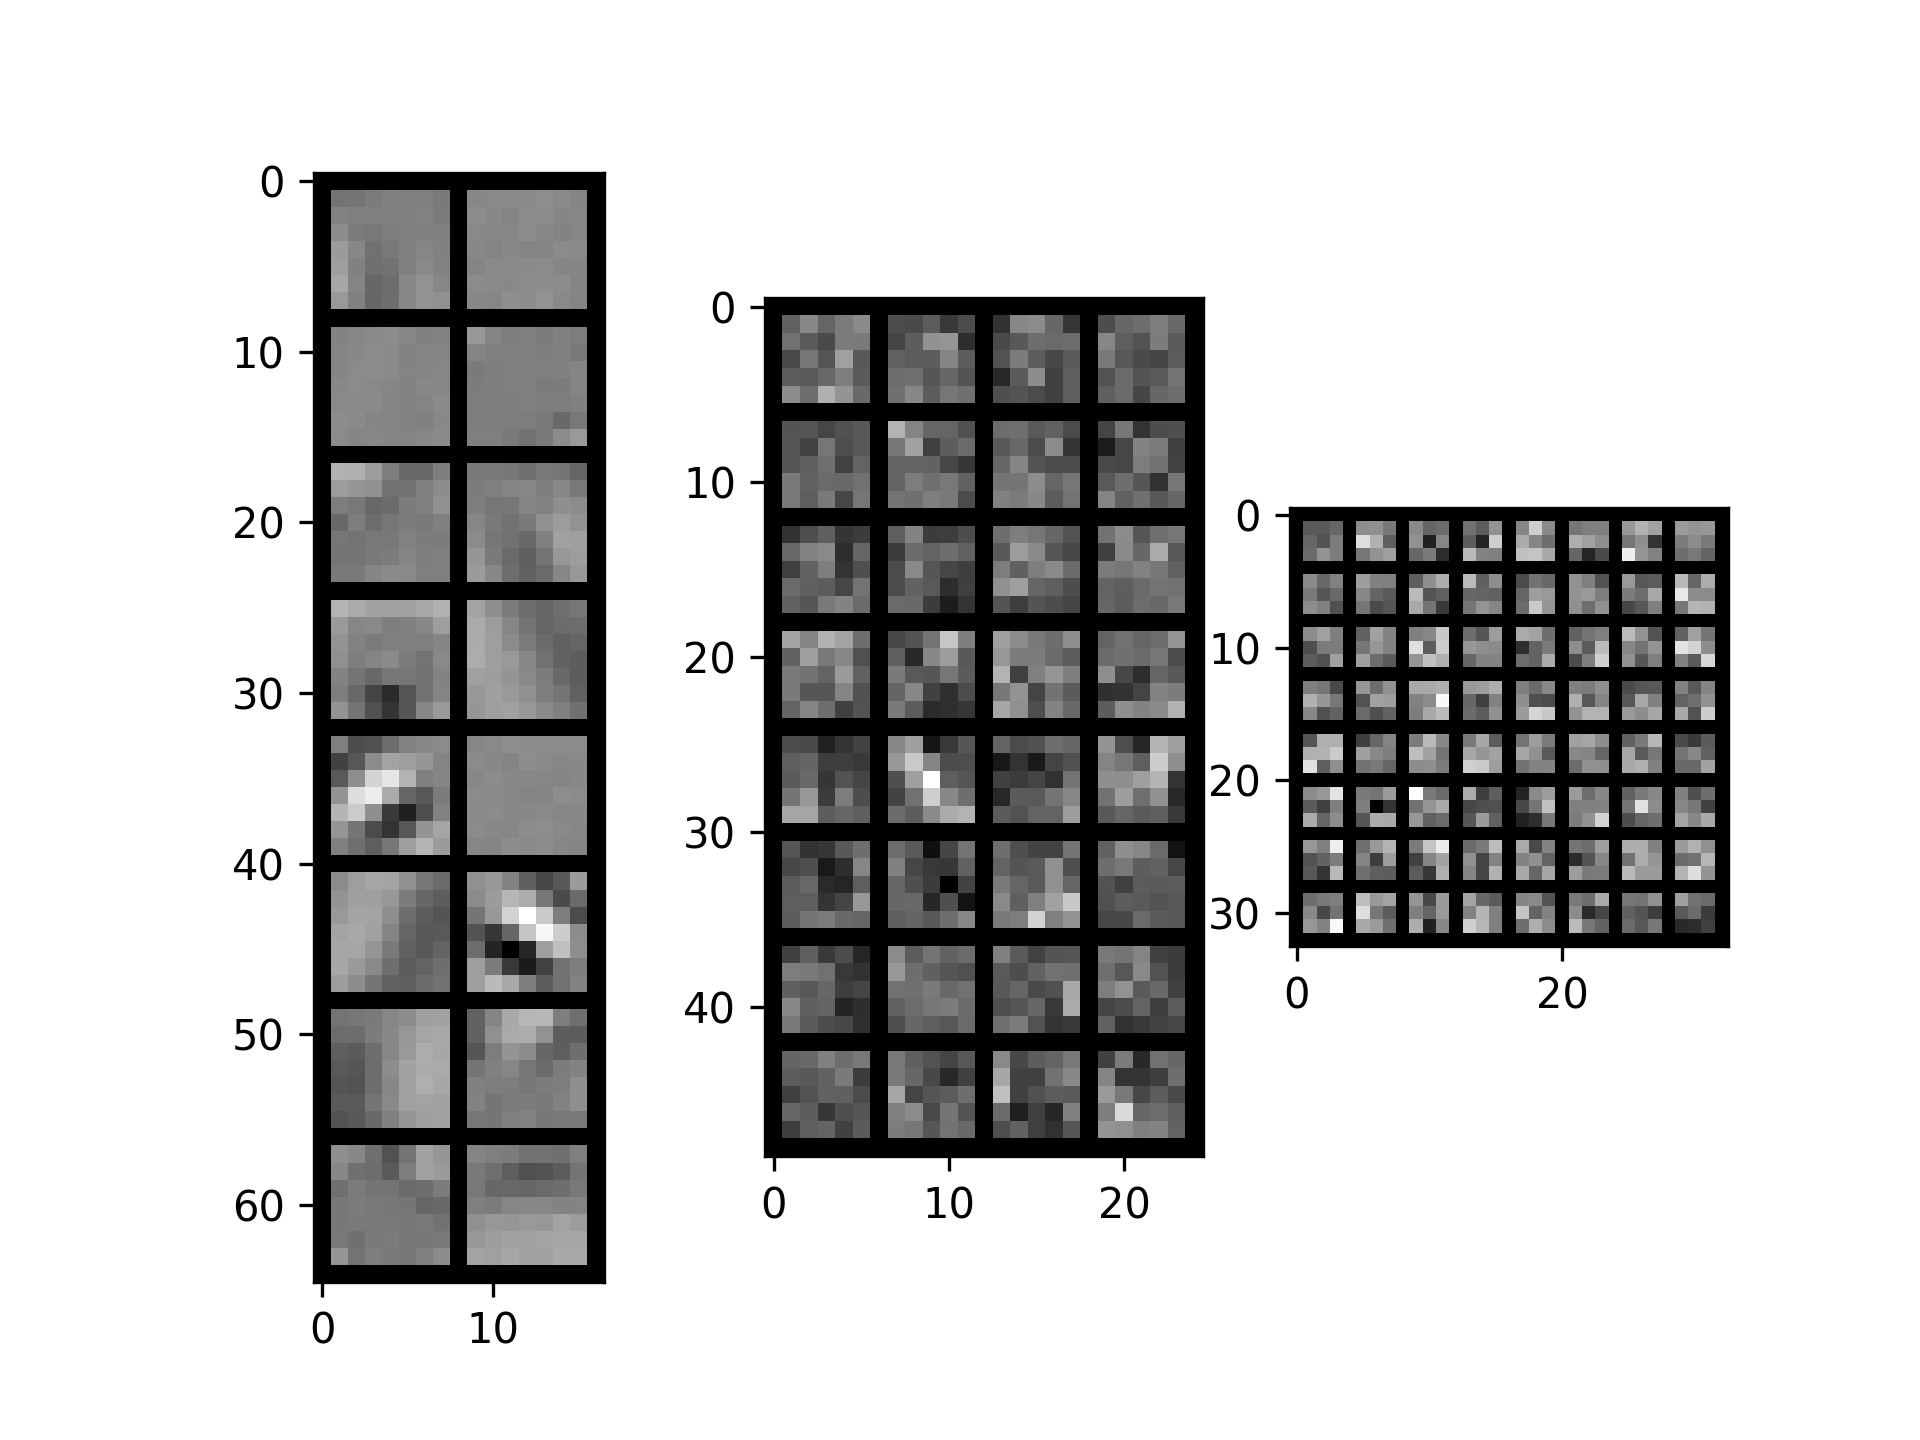
\includegraphics[width=\linewidth]{4.CNN_2500_sample/CNN_filters.png}
    \caption{CNN filters.}
    \label{fig:image1}
  \end{minipage}
  \hspace{0.5cm}
  \begin{minipage}[b]{\weight\linewidth}
    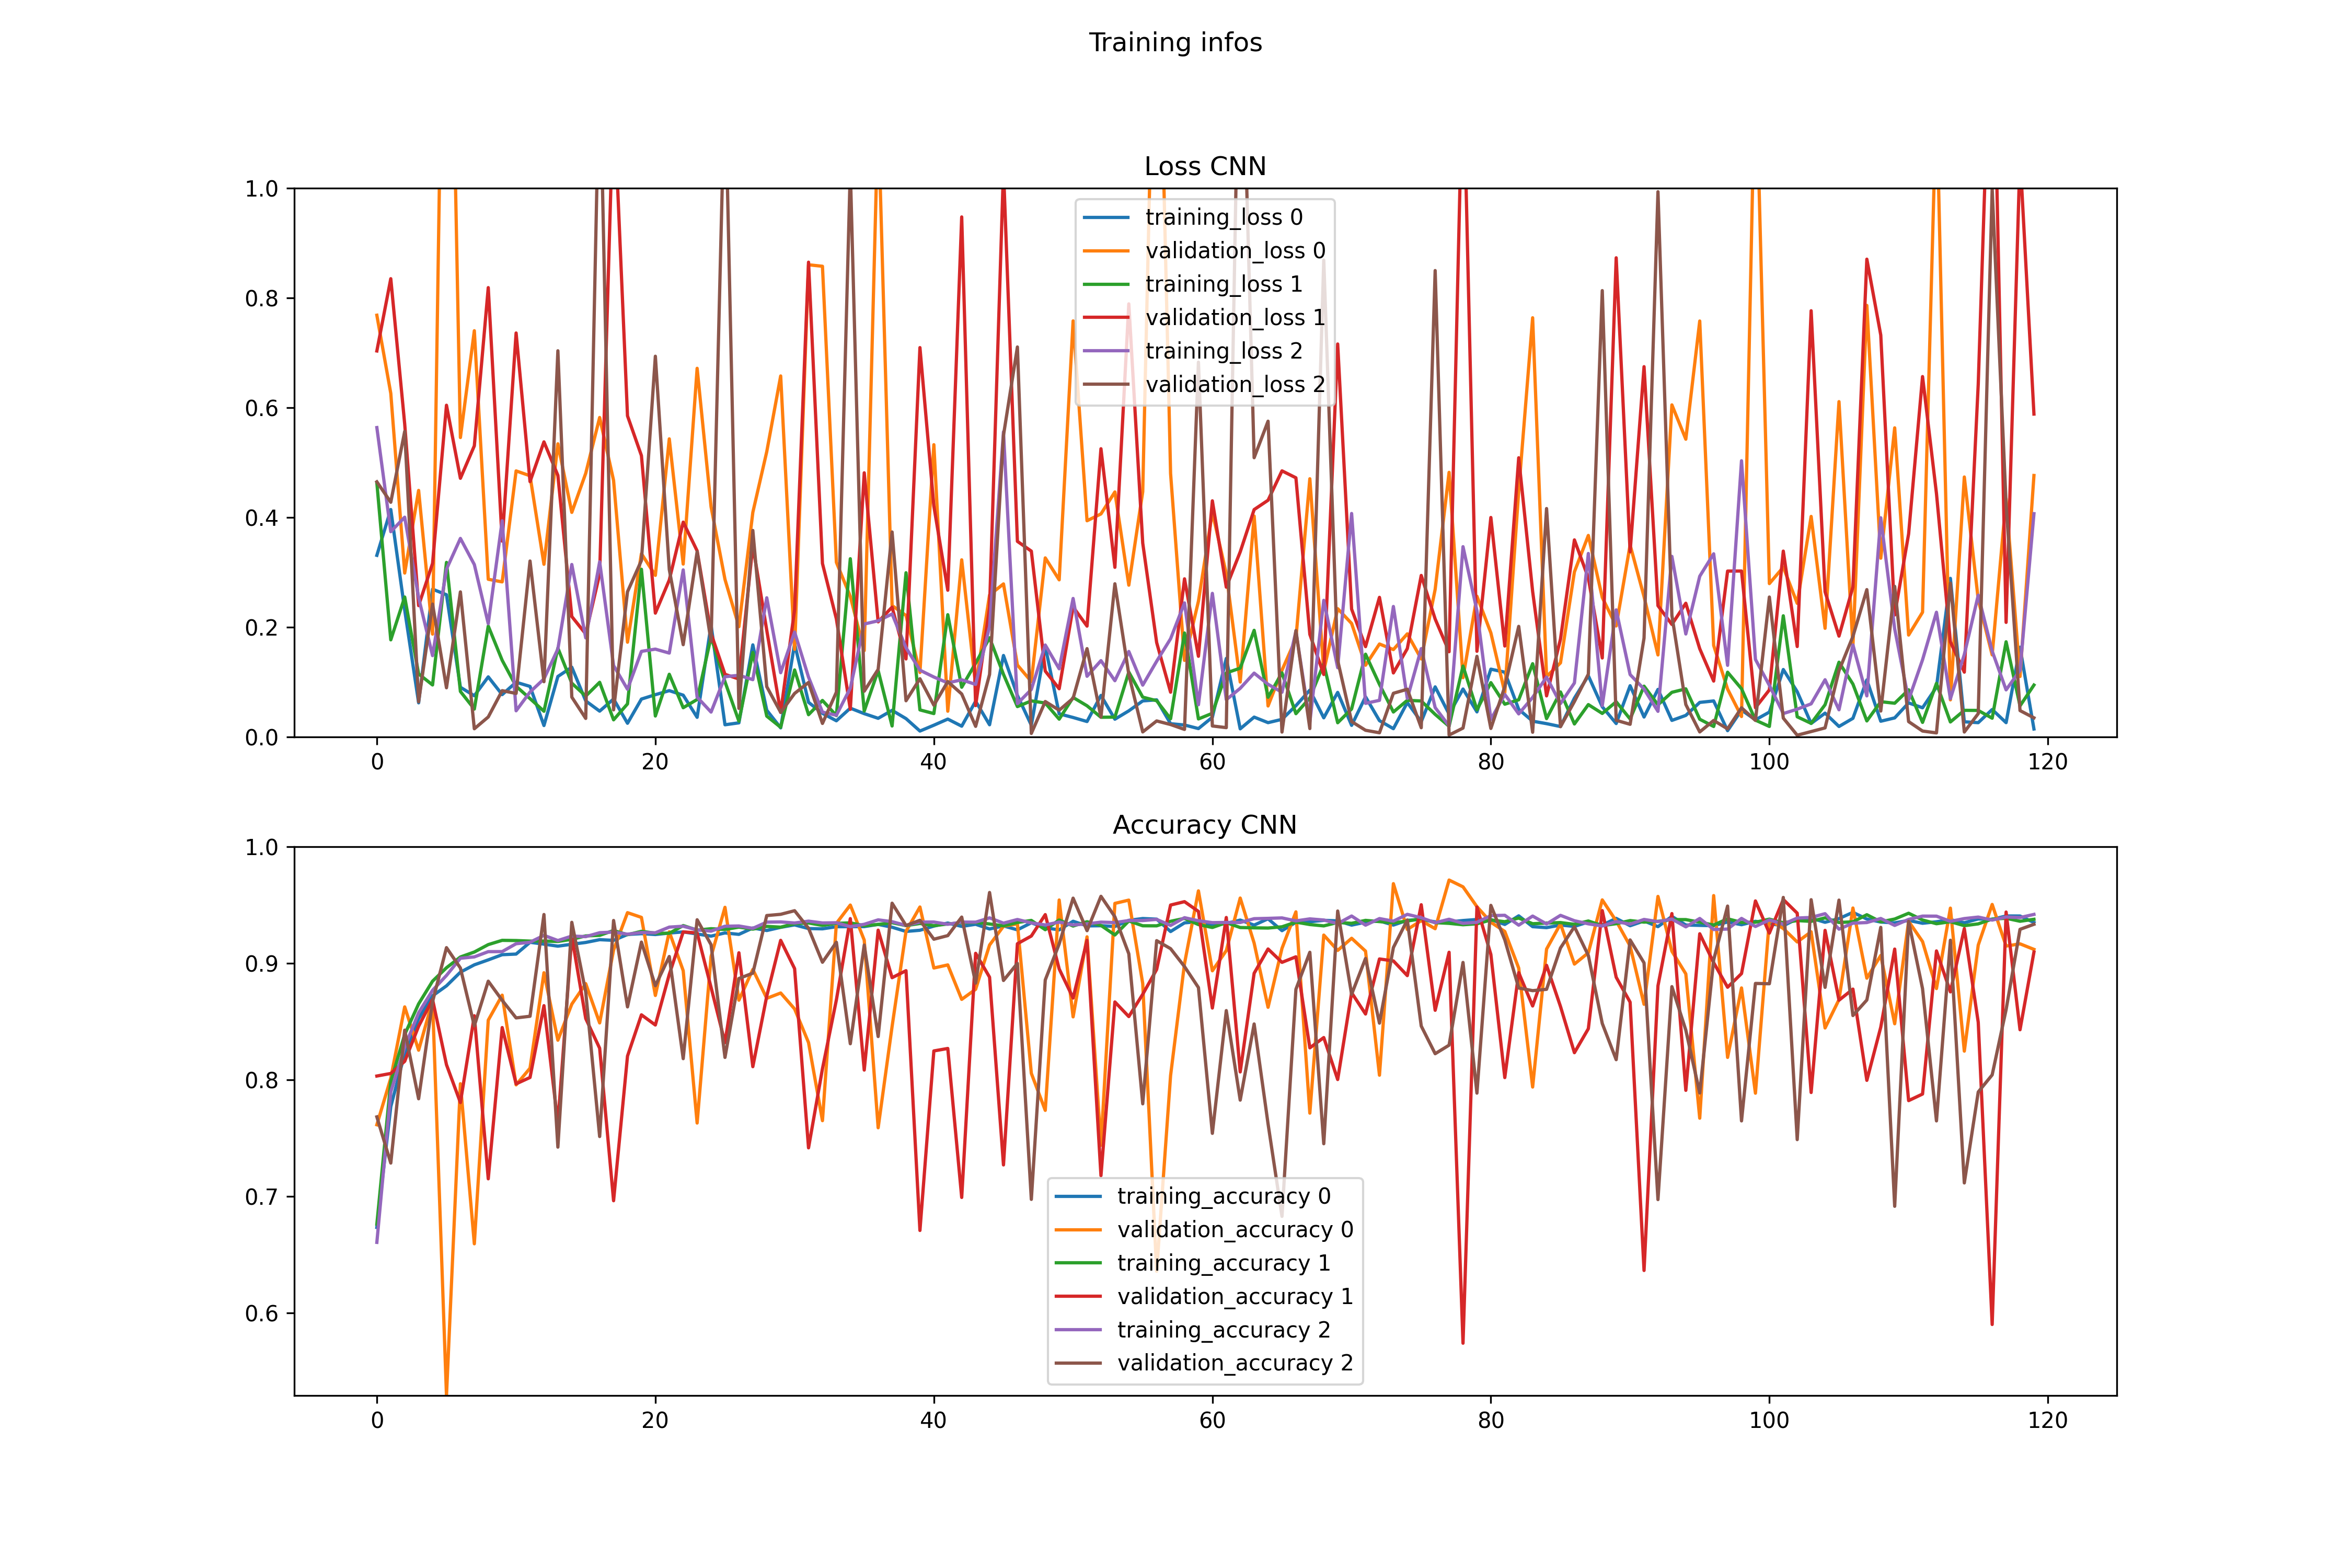
\includegraphics[width=\linewidth]{4.CNN_2500_sample/training_infos.png}
    \caption{Loss and Validation graphs.}
    \label{fig:image2}
  \end{minipage}
\end{figure}\\
The \textbf{accuracy} reached in test is $0.87$.\\
\pagebreak

For the NN executions with agumentation we have these results:
\begin{figure}[ht!]
  \centering
  \begin{minipage}[b]{\weight\linewidth}
    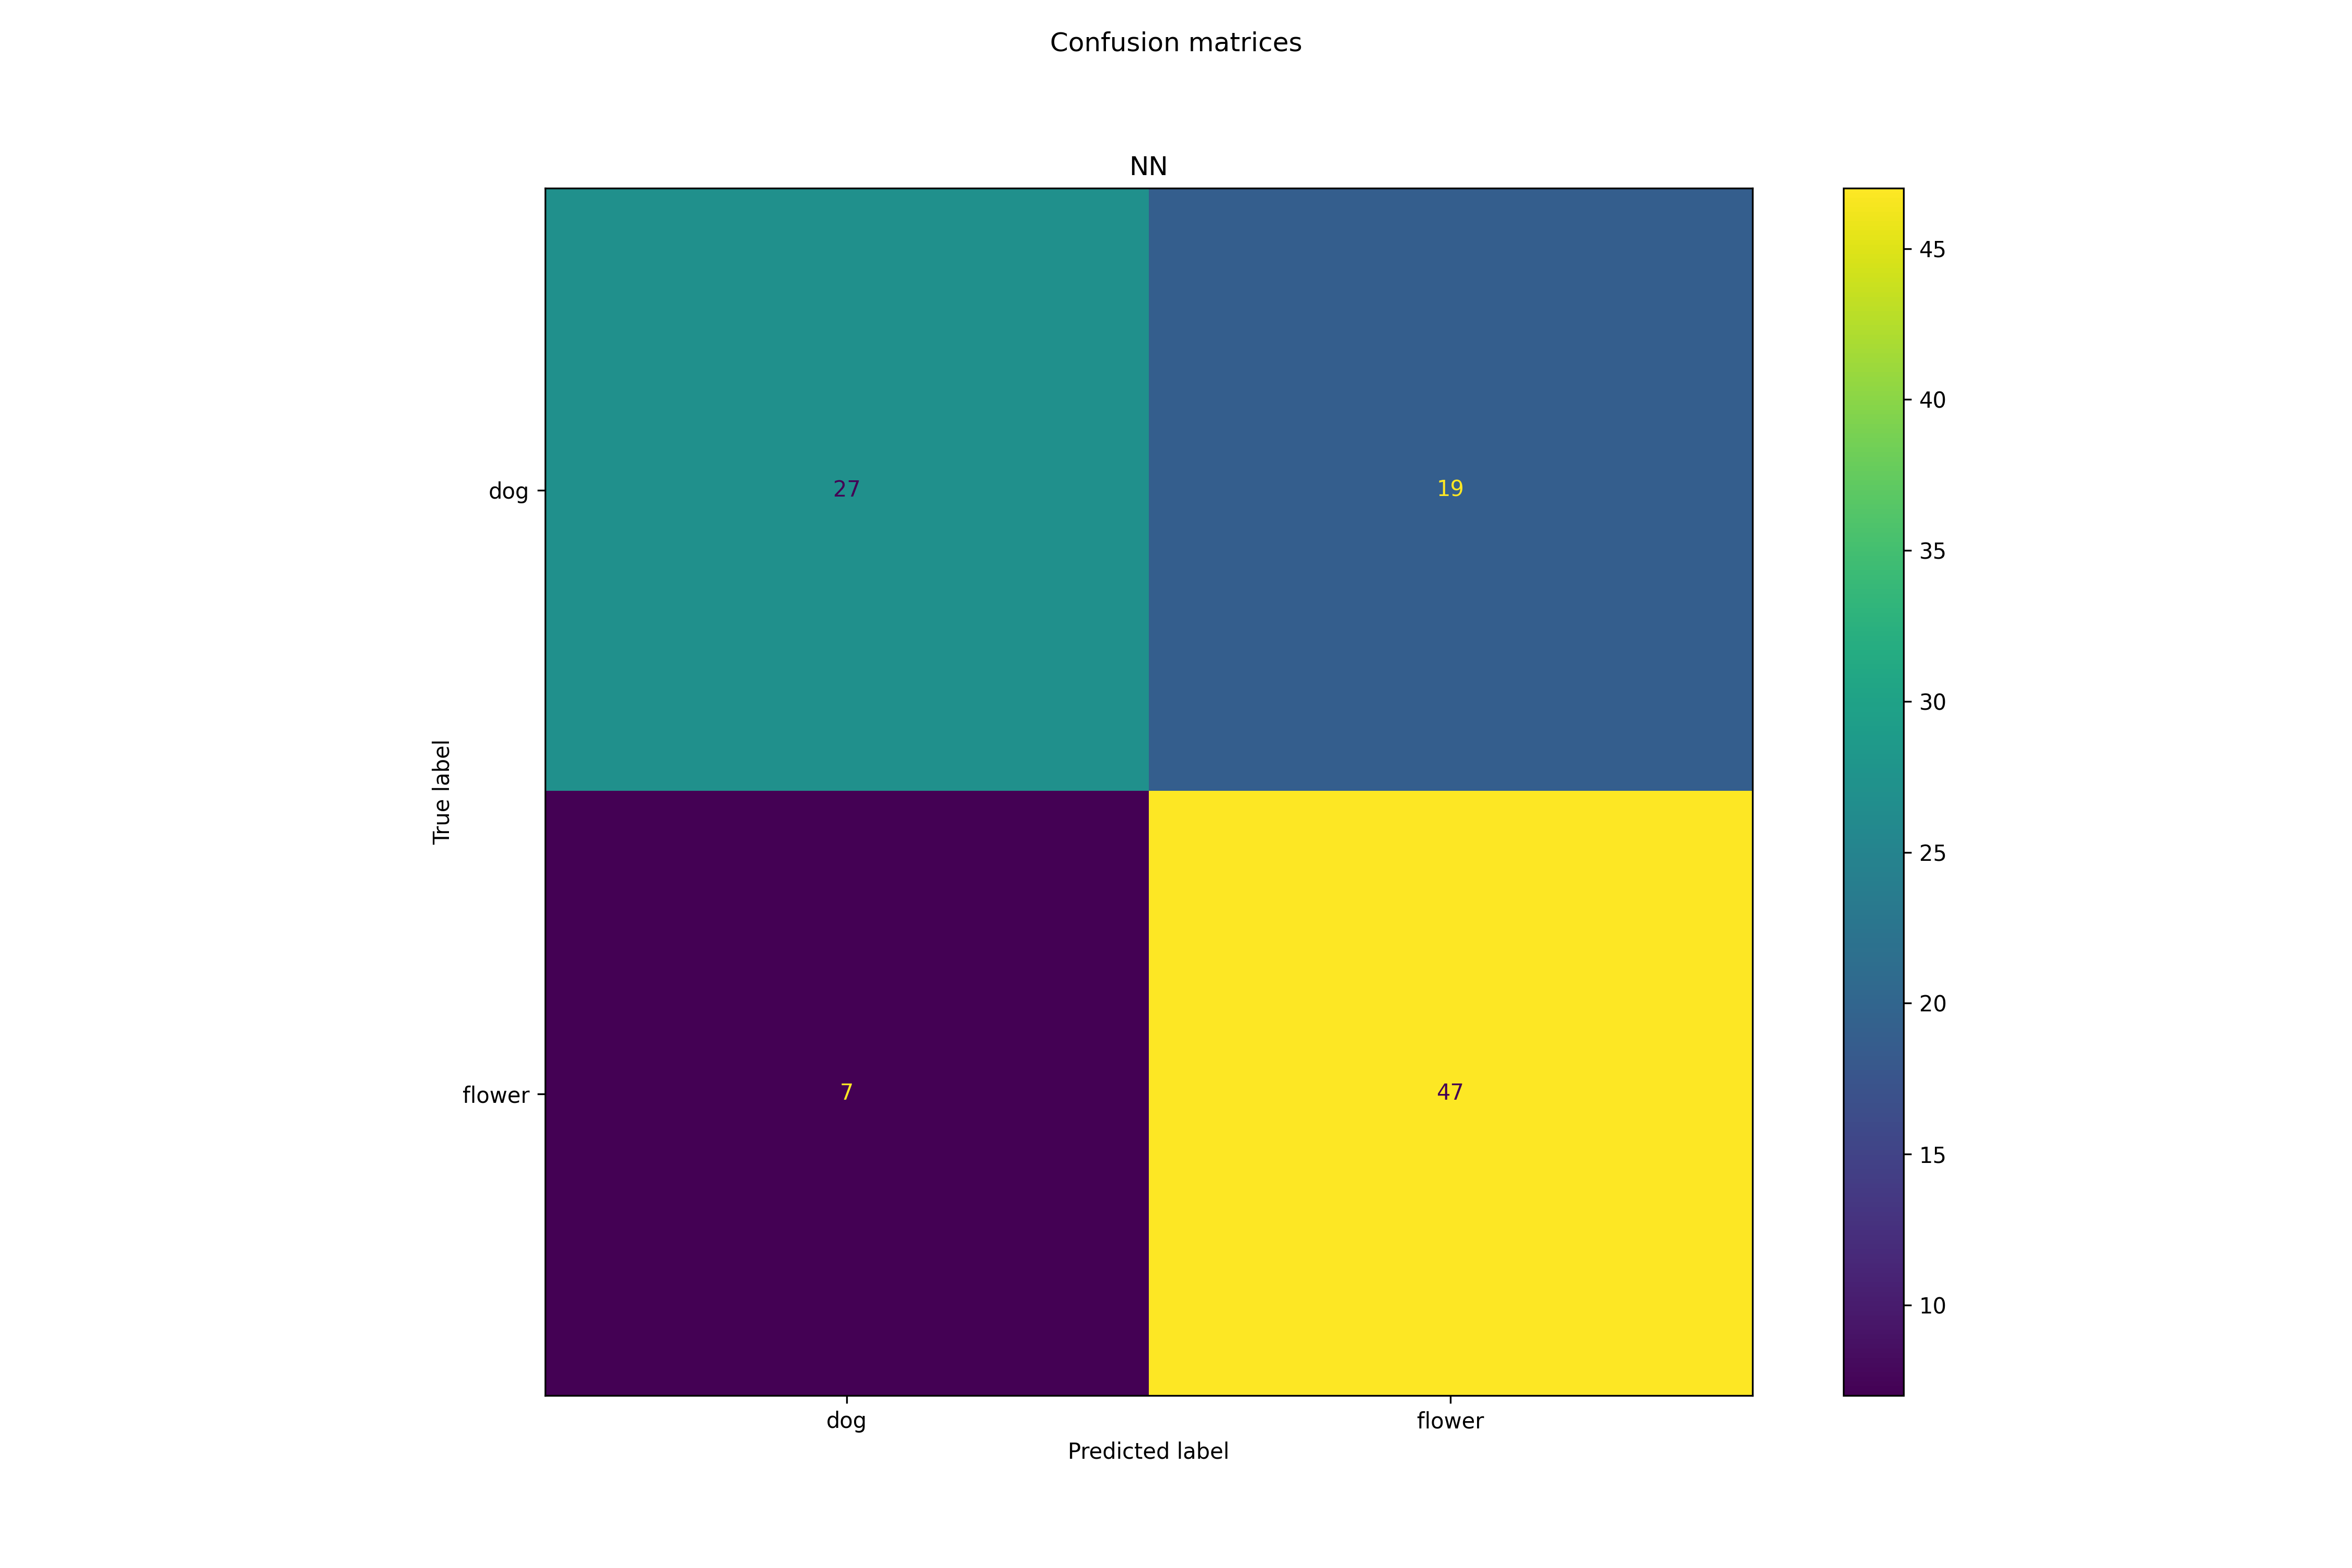
\includegraphics[width=\linewidth]{1.augmentationNN/conf_mat.png}
    \caption{Confusion matrix.}
    \label{fig:image1}
  \end{minipage}
  \hspace{0.5cm}
  \begin{minipage}[b]{\weight\linewidth}
    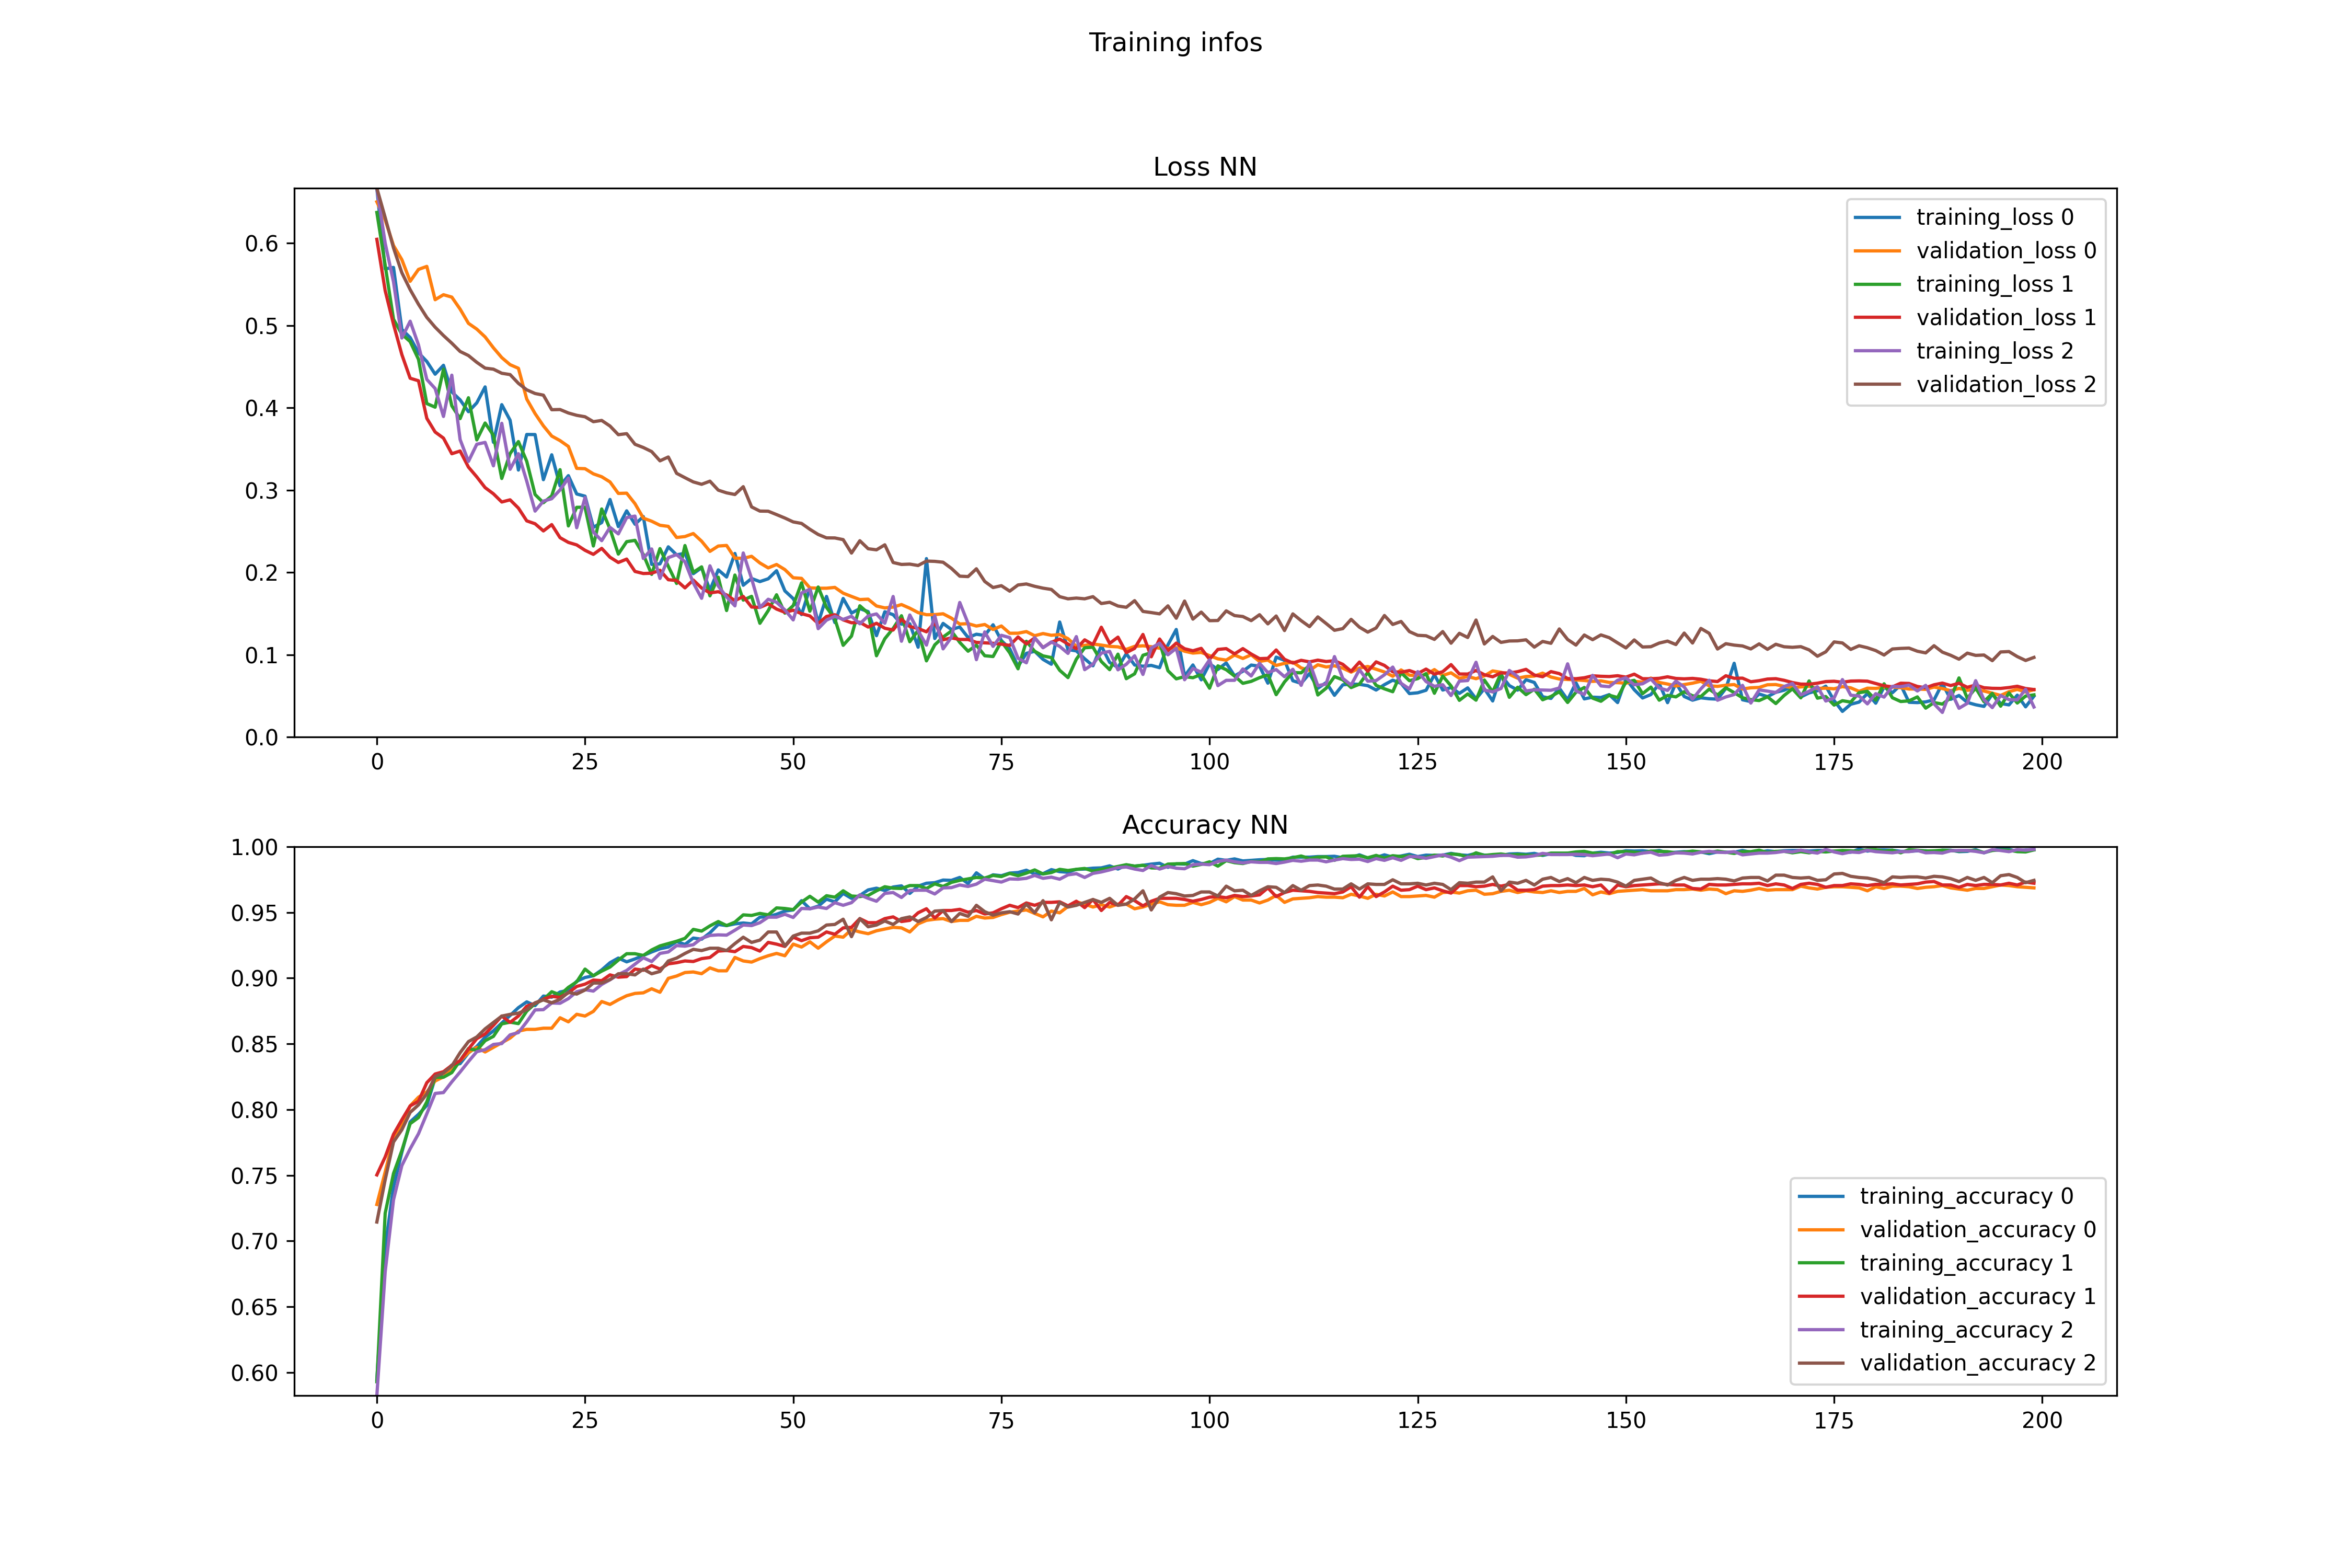
\includegraphics[width=\linewidth]{1.augmentationNN/training_infos.png}
    \caption{Loss and Validation graphs.}
    \label{fig:image2}
  \end{minipage}
\end{figure}\\
The \textbf{accuracy} reached in test is $0.74$.\\

\pagebreak

For the NN executions without agumentation we have these results:
\begin{figure}[ht!]
  \centering
  \begin{minipage}[b]{\weight\linewidth}
    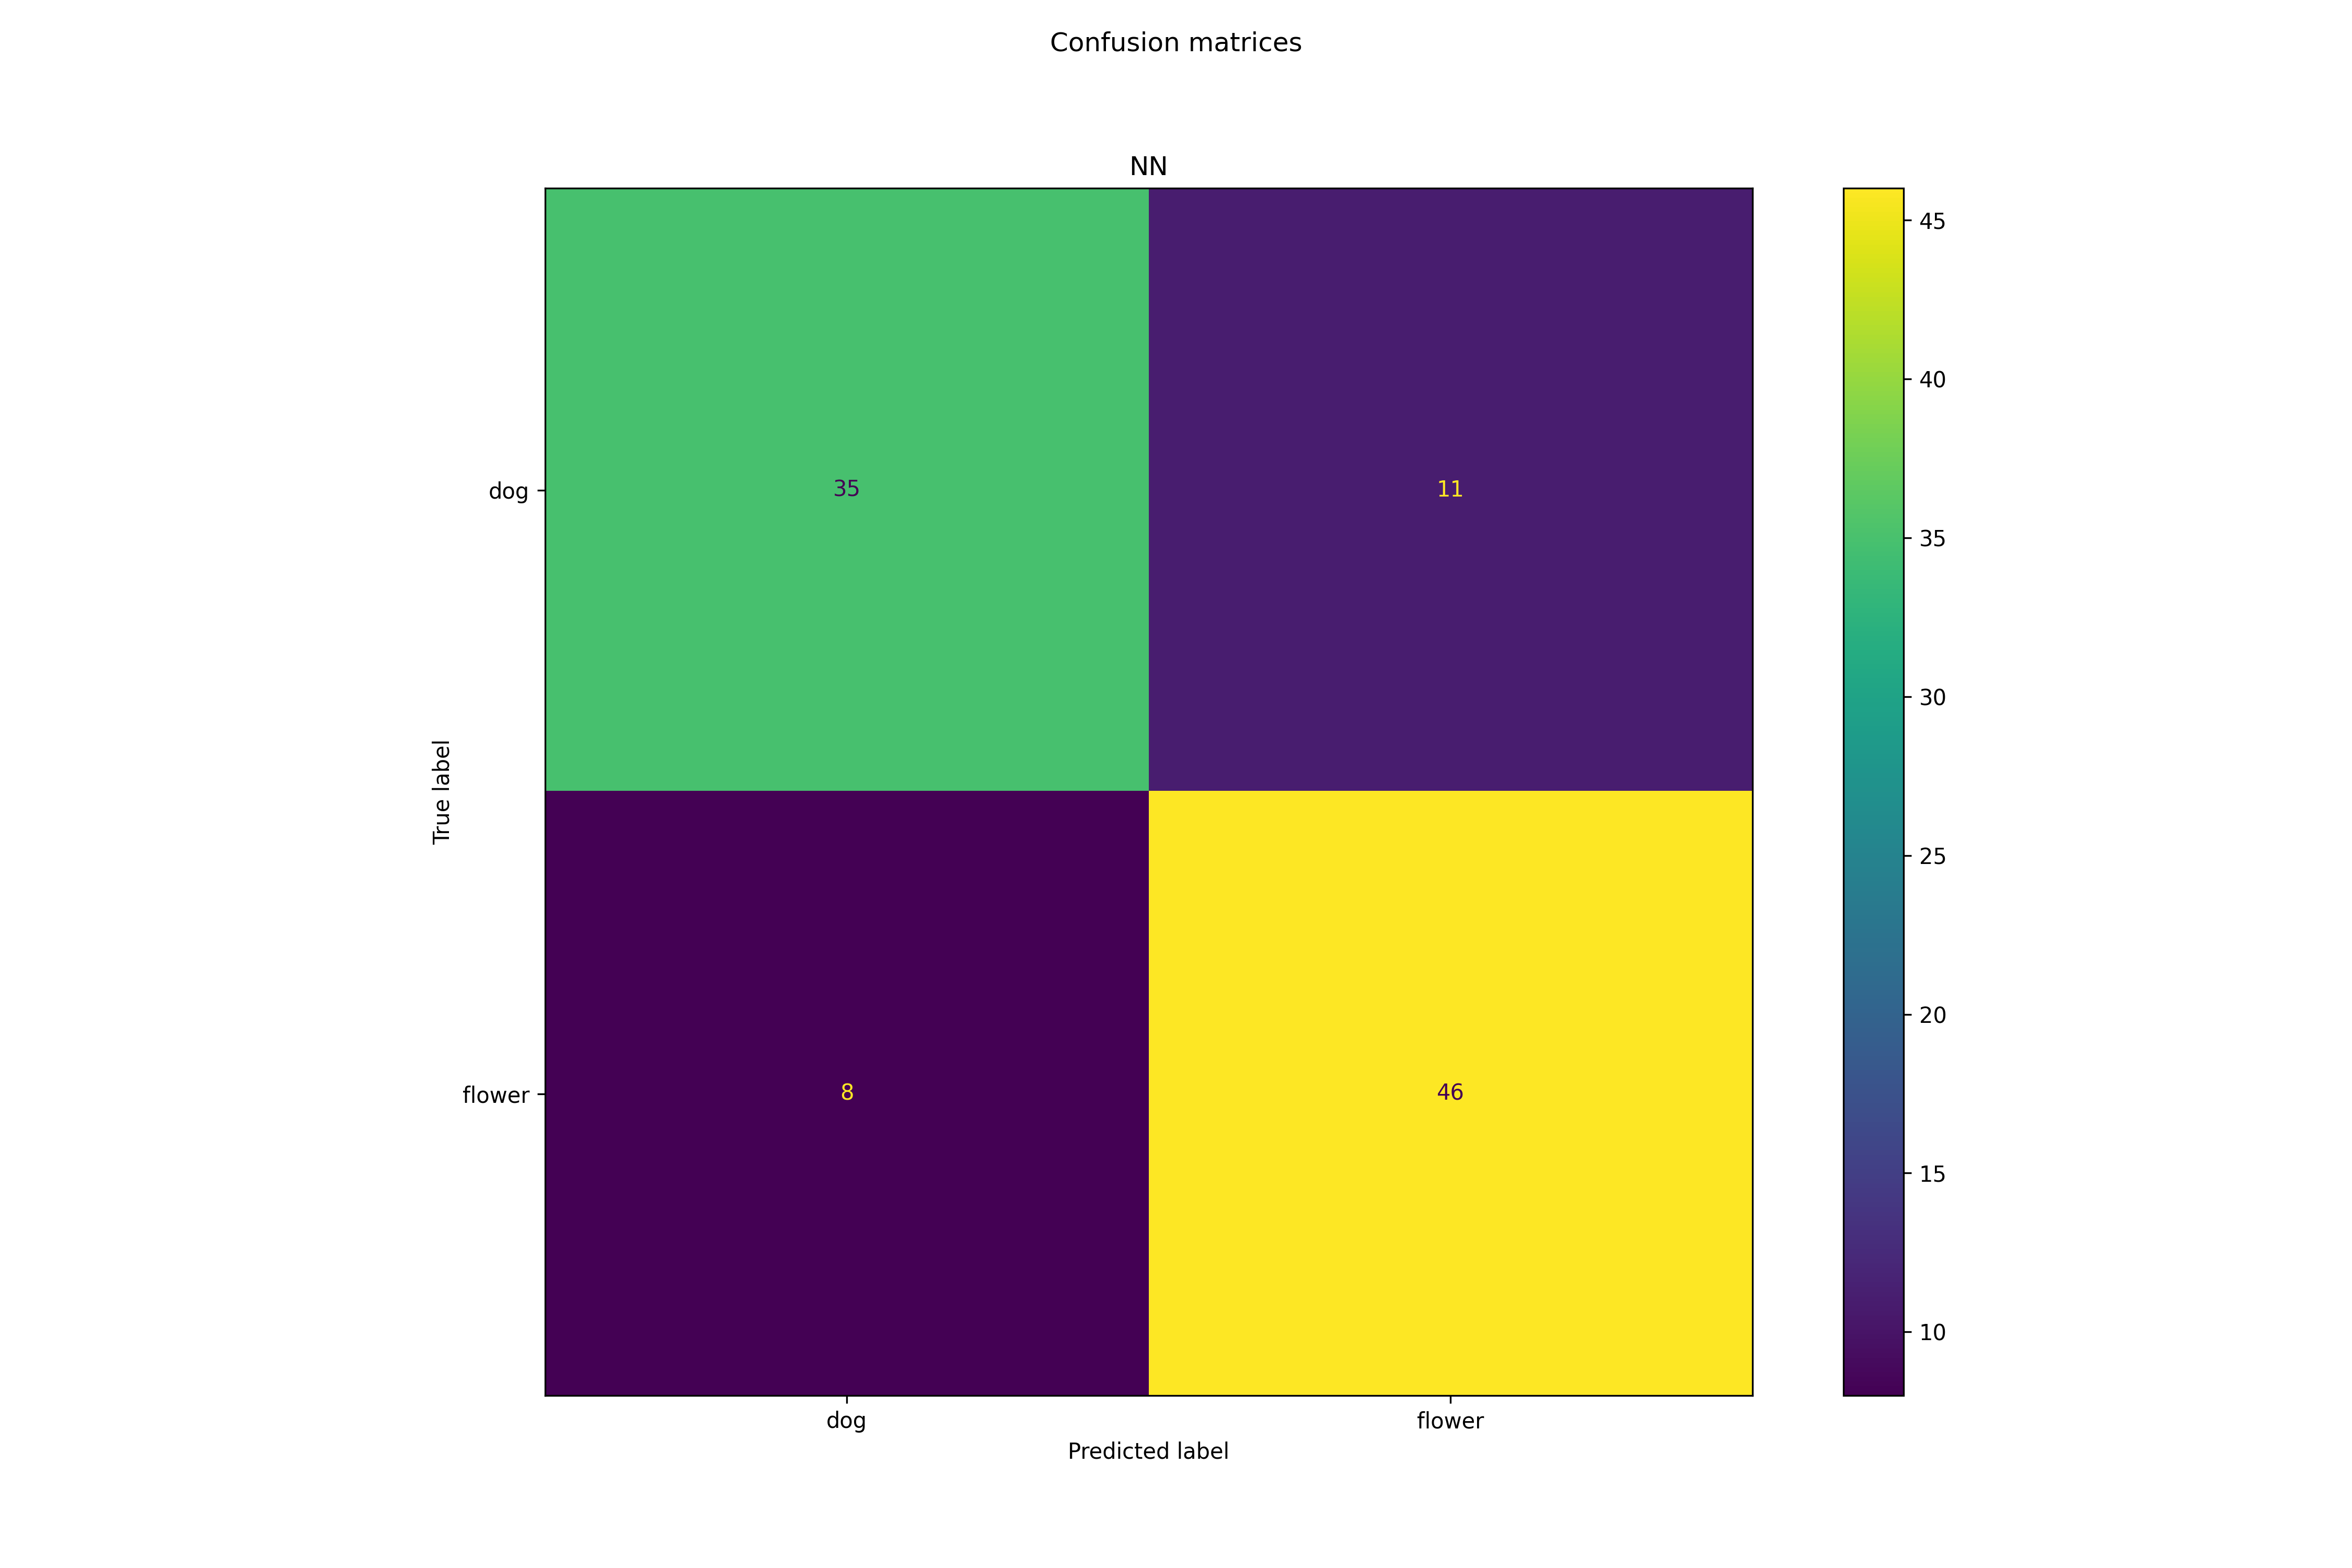
\includegraphics[width=\linewidth]{2.senza_augmentationNN/conf_mat.png}
    \caption{Confusion matrix.}
    \label{fig:image1}
  \end{minipage}
  \hspace{0.5cm}
  \begin{minipage}[b]{\weight\linewidth}
    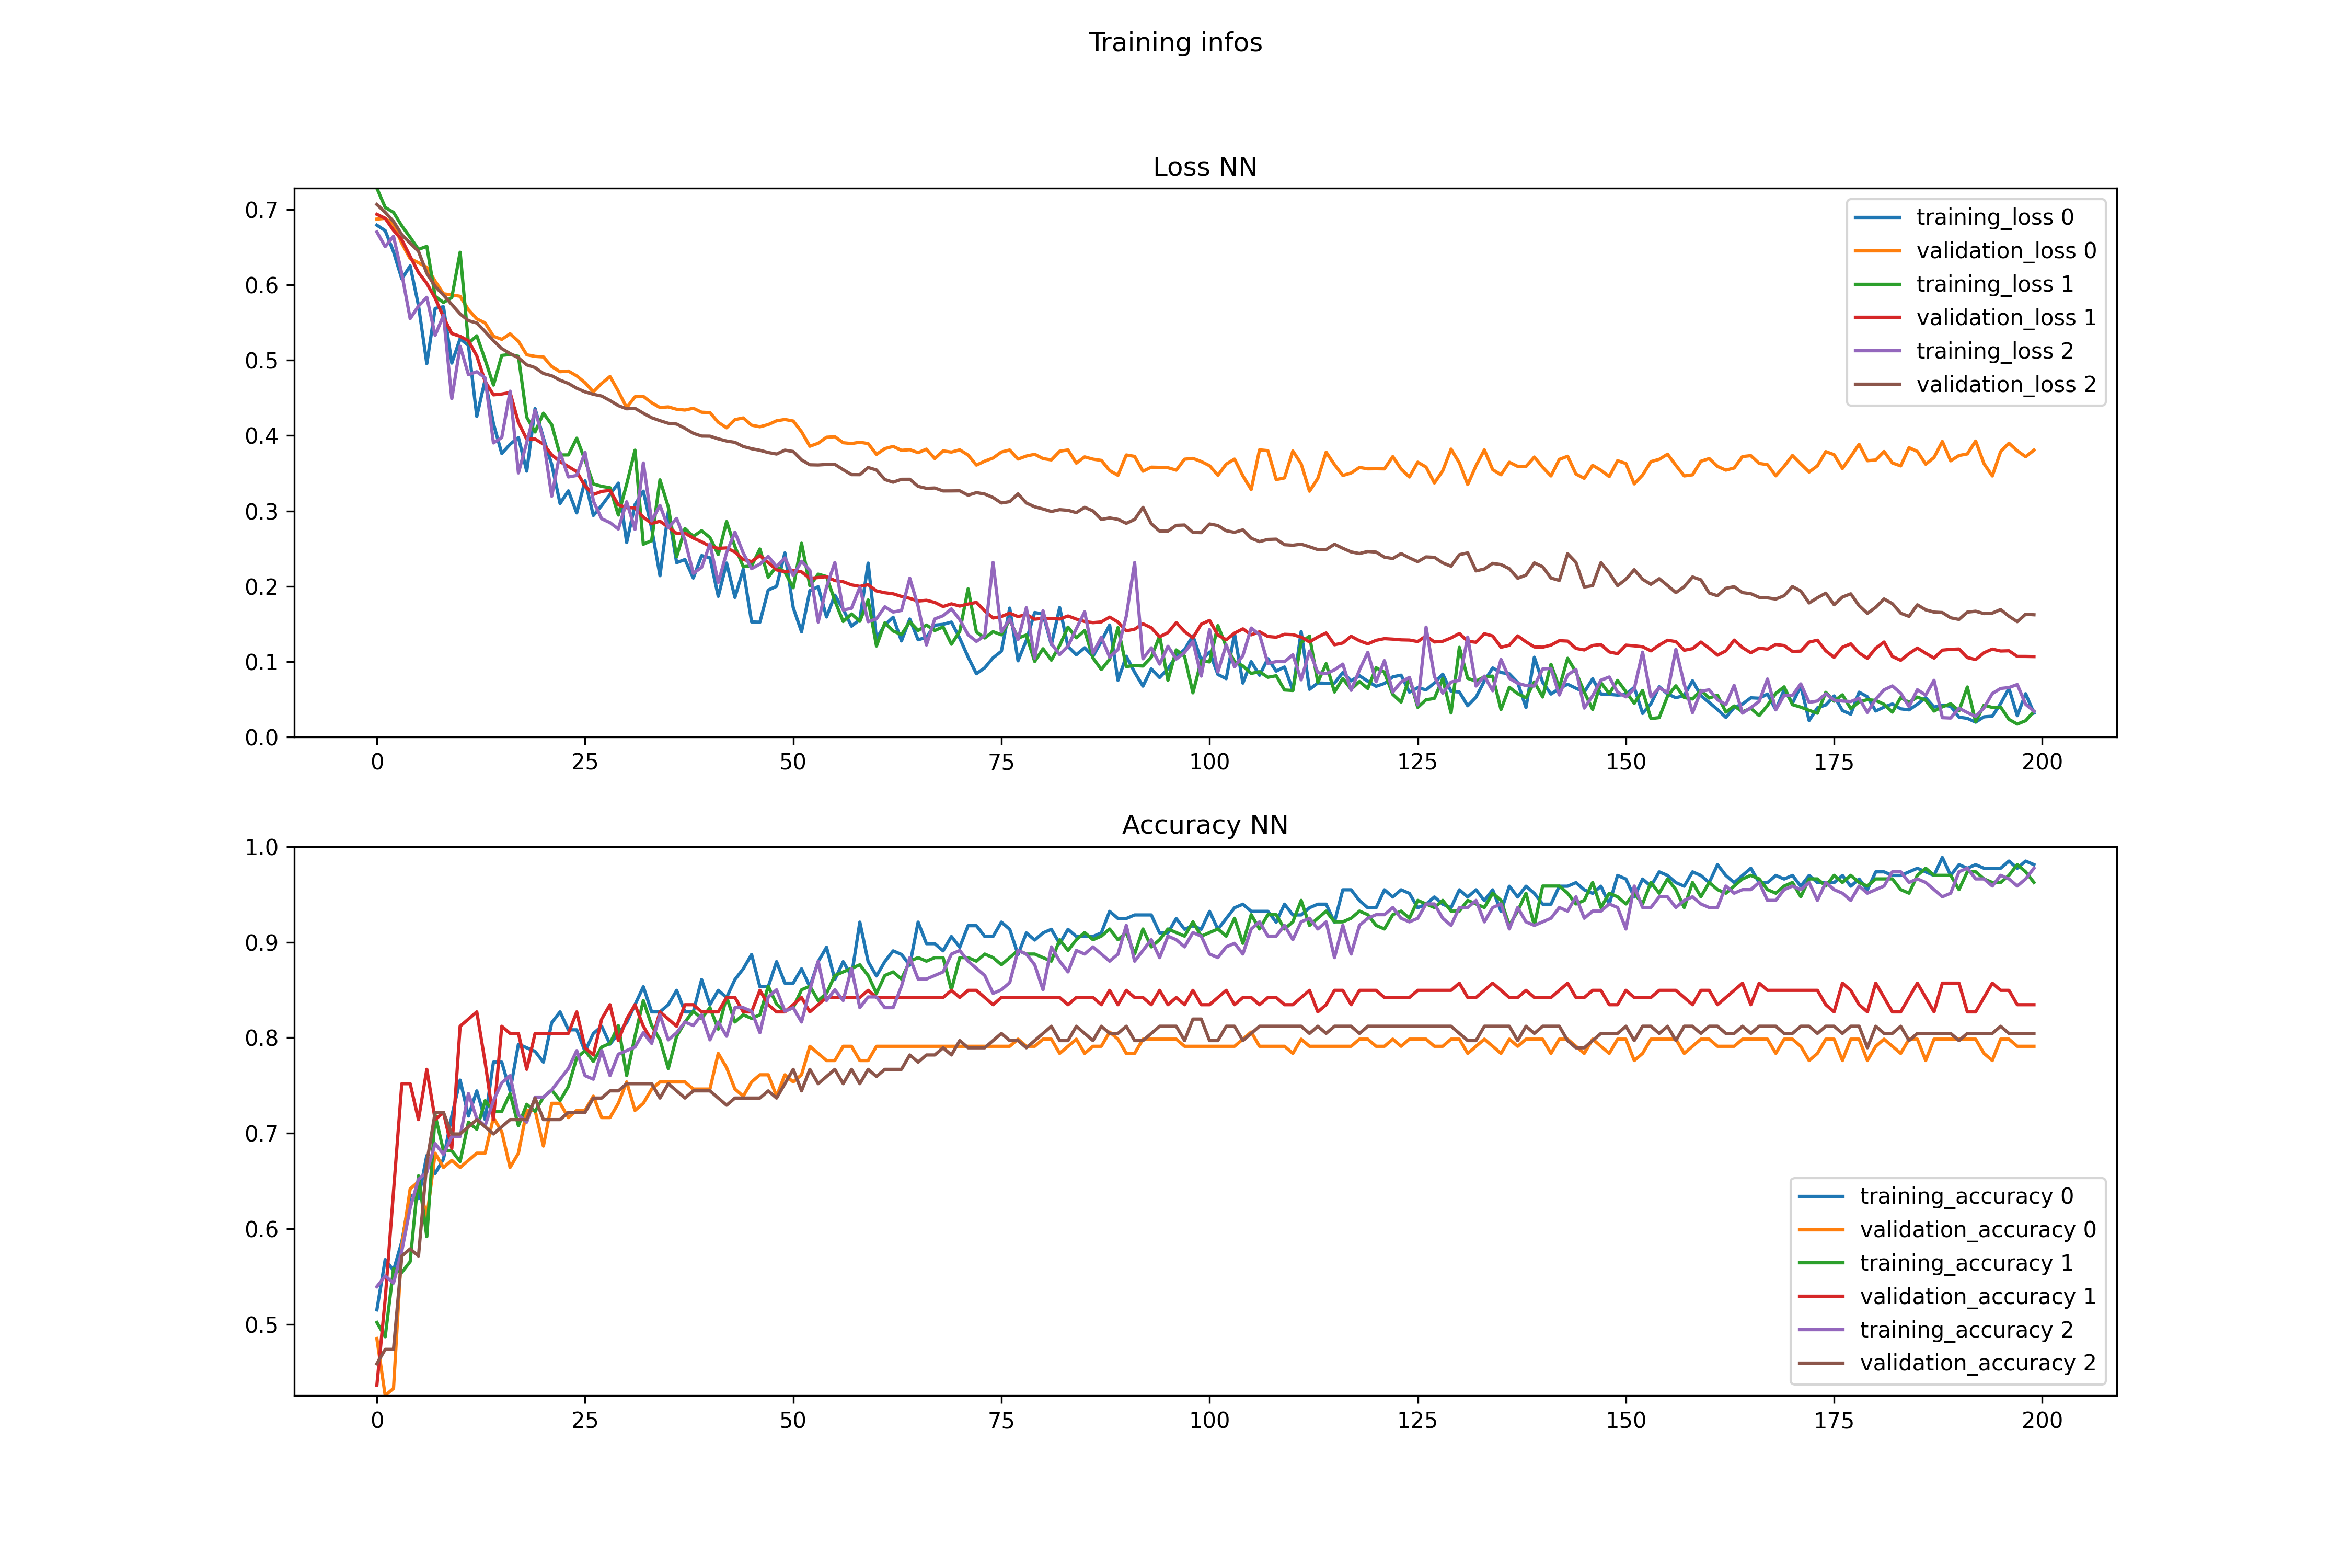
\includegraphics[width=\linewidth]{2.senza_augmentationNN/training_infos.png}
    \caption{Loss and Validation graphs.}
    \label{fig:image2}
  \end{minipage}
\end{figure}\\
The \textbf{accuracy} reached in test is $0.81$.\\



\end{document}